
%(BEGIN_QUESTION)
% Copyright 2011, Tony R. Kuphaldt, released under the Creative Commons Attribution License (v 1.0)
% This means you may do almost anything with this work of mine, so long as you give me proper credit

An Emerson Smart Wireless Gateway is installed to act as the link between a set of {\sl Wireless}HART field instruments and a PLC host system.  The PLC communicates with the Gateway using Modbus digital codes over an RS-485 serial data network cable, with the PLC acting as master and the Gateway acting as slave.  24 VDC is supplied through another cable to power the Gateway.  

For some reason, the PLC is unable to communicate with the {\sl Wireless}HART Gateway unit in this brand-new installation.  You are summoned to diagnose the problem, and the first thing you notice on the PLC is the ``Transmit'' LED for the serial Modbus port blinking rapidly:

$$\includegraphics[width=15.5cm]{i03606x01.eps}$$

Which {\it one} multimeter measurement would show you whether or not a DC power wiring fault anywhere in the system was the problem?  Identify the two terminals to measure between in this circuit, and the proper setting for your multimeter (e.g. AC milliamps, ohms, diode check, etc.) when performing the test.

\vskip 20pt

Which {\it one} multimeter measurement would show you whether or not a network wiring fault was interrupting Modbus data signals?  Identify the two terminals to measure between in this circuit, and the proper setting for your multimeter (e.g. AC milliamps, ohms, diode check, etc.) when performing the test.

\vskip 20pt

If both of these tests turn out successful (i.e. there is both DC power and data signal present), identify \underbar{one} other problem that might account for the lack of communication between the Gateway and the PLC.

\underbar{file i03606}
%(END_QUESTION)





%(BEGIN_ANSWER)

\noindent
{\bf 2 points:} Measure DC voltage between terminals (+) and ($-$) on the Gateway.

\vskip 10pt

\noindent
{\bf 2 points:} Measure AC voltage between terminals (A) and (B) on the Gateway.

\vskip 10pt

\noindent
{\bf 6 points:} Possible problems include, but are not limited to: Modbus wires (A/B) swapped, incorrect bit rate, incorrect number of stop bits, incorrect parity.

%(END_ANSWER)





%(BEGIN_NOTES)

{\bf This question is intended for exams only and not worksheets!}

%(END_NOTES)


